% !TEX program  = xelatex
\documentclass[a4paper]{article}
\usepackage{amsmath}
\usepackage{amssymb}
\usepackage{enumerate}
\usepackage{amstext}
\usepackage{ctex}
%\usepackage{braket}
\usepackage[european]{circuitikz}
\usepackage{multirow}
\usepackage{graphicx}
\usepackage{subfig}
\usepackage{float}
\usepackage{url}
%\usepackage[table,xcdraw]{xcolor}
\usepackage{colortbl}
\usepackage{geometry}
\geometry{left=2.5cm,right=2.5cm,bottom=2.5cm,top=2.5cm}

\title{模电实验报告9:LC正弦波振荡和选频放大电路实验}
\author{xy\quad 学号\quad 匡亚明学院}
\date{2019年2月29日}
\begin{document}
\maketitle
\bibliographystyle{unsrt}
%--------main-body------------

\section{实验目的}
\begin{enumerate}
\item 研究、学习LC正弦波振荡器的特性。
\item 研究、学习LC选频放大电路的特性。
\end{enumerate}

\section{实验仪器}
示波器、信号发生器、交流毫伏表、数字万用表。

\section{预习内容}
\begin{enumerate}
\item 复习LC正弦波振荡器的基础知识。
\item 复习LC选频放大电路的基础知识。
\end{enumerate}

\section{实验内容}
\subsection{电容三端式LC振荡器}
\subsubsection{原理}
电路如图(\ref{fig1})所示。

\begin{figure}[!h]
\centering
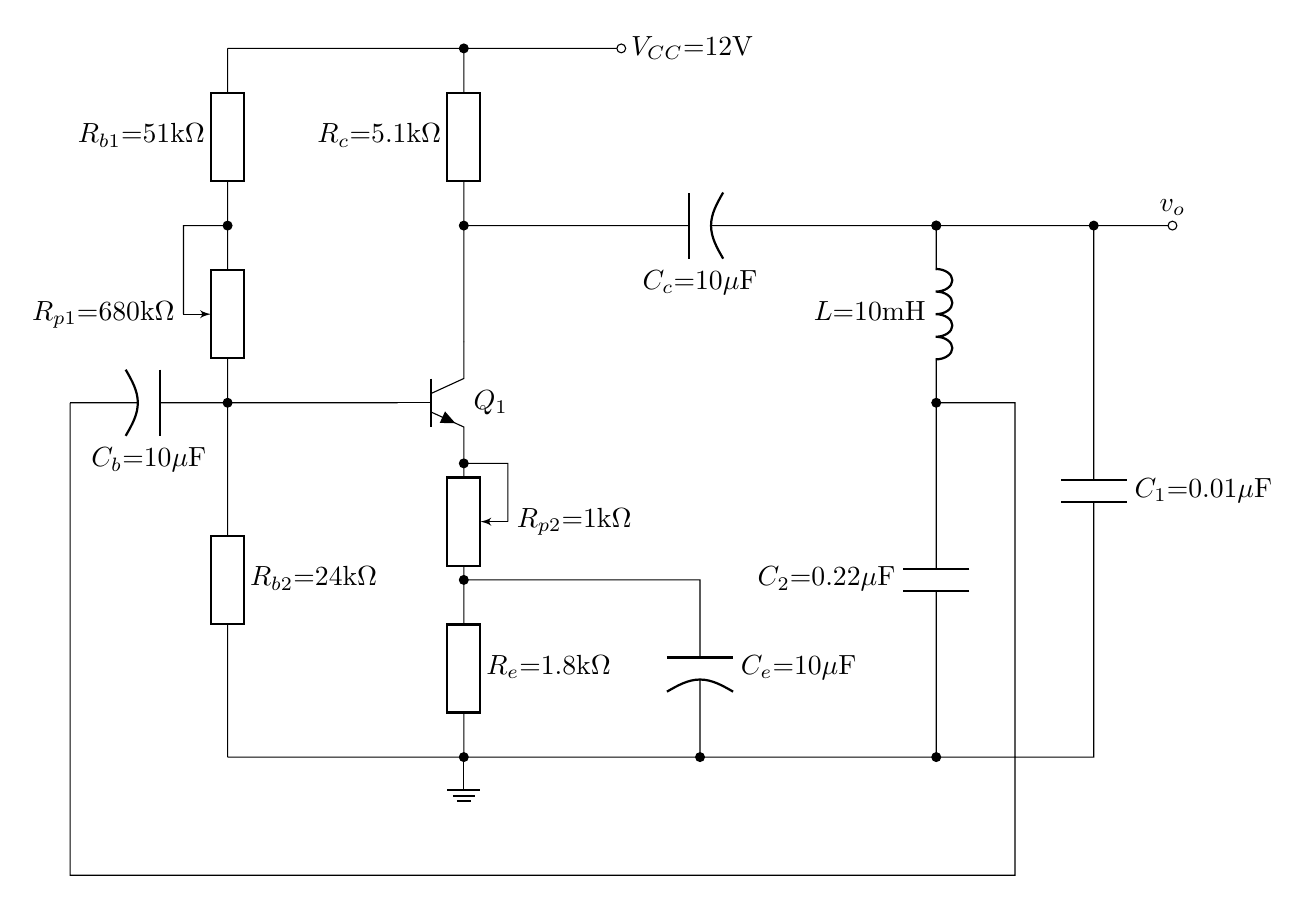
\begin{tikzpicture}[x = 2cm, y = 1.5cm]
    \draw
        (2,3) to [pC, l_= $C_b{=}10\mu\text{F}$] (3,3) node[circ]{} to [R, l = $R_{b2}{=}24\text{k}\Omega$] (3,0)
        (3,3) to [pR, l = $R_{p1}{=}680\text{k}\Omega$, n = PR1, -*] (3,4.5) to [R, l = $R_{b1}{=}51\text{k}\Omega$] (3,6)
        (3,4.5) -| (PR1.wiper)
        (4.5,3) node[npn](NPN){}
        (3,3) to [-] (NPN.B)
        (NPN.E) to [pR, l = $R_{p2}{=}1\text{k}\Omega$, n = PR2] (4.5, 1.5) to [R, l = $R_{e}{=}1.8\text{k}\Omega$] (4.5,0)
        (PR2.wiper) |- (NPN.E) node[circ]{}
        (NPN.C) to [-] (4.5,4.5) to [R, l = $R_c{=}5.1\text{k}\Omega$] (4.5,6) to [-] (3,6)
        (4.5,6) to [short, *-o] (5.5,6) node[right]{$V_{CC}{=}12\text{V}$}
        (7.5,4.5) to [pC, *-*, l = $C_c{=}10\mu\text{F}$] (4.5,4.5)
        (7.5,4.5) to [short, *-*] (8.5,4.5) to [C, l=$C_1{=}0.01\mu\text{F}$] (8.5,0) to [short, -*] ++(-1,0)
        (8.5,4.5) to [short, -o] (9,4.5)
        (7.5,4.5) to [american inductor, l_= $L{=}10\text{mH}$] (7.5,3) to [C, l_=$C_2{=}0.22\mu\text{F}$] (7.5,0)
        (6,0) to [pC, l_= $C_e{=}10\mu\text{F}$] (6,1.5) -- ++(-1.5,0) node[circ]{}
        (3,0) to [short, -*] (4.5,0) to [short, -*] (6,0) to [-] (7.5,0)
        (7.5,3) node[circ]{} -- ++(0.5,0) -- ++(0,-4) -| (2,3)
        (4.5,0) node[ground](GND){}
        {[anchor = south] (9,4.5) node{$v_o$}}
        {[anchor = west] (4.5,3) node{$Q_1$}}
    ;
    \end{tikzpicture}
\caption{电容三端式LC振荡器}\label{fig1}
\end{figure}

这是一个电容三端式LC振荡器,其简化的原理示意图如图(\ref{fig2})。

\begin{figure}[!h]
\centering
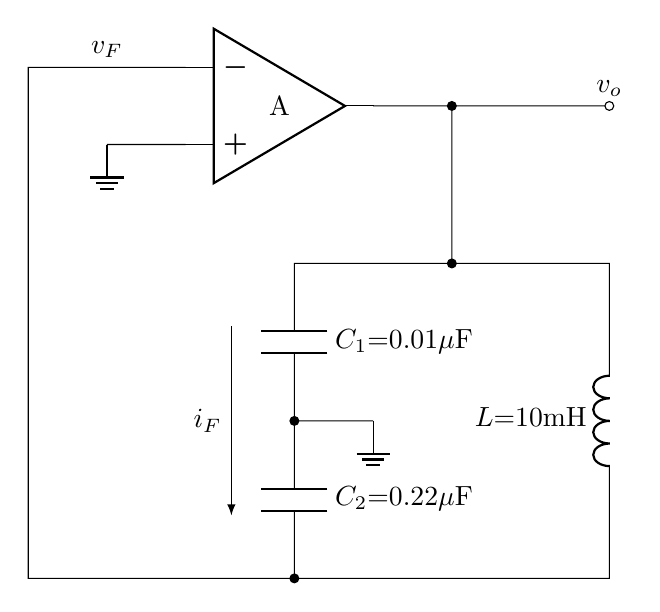
\begin{tikzpicture}[x = 2cm, y = 2cm]
    \draw (0,0) node[op amp](AMP){} node[]{A};
    \draw let \p1 = (AMP.-), \p2 = (AMP.+), \p3 = (AMP.out) in
    (AMP.+) -- ++(-0.5,0) node[ground]{}
    (AMP.out) -- ++(0.5,0) node[circ](OUT){} to [short, -o] ++(1,0)  node[anchor = south]{$v_o$}
    (OUT) -- ++(0,-1) node[circ]{} -- ++(-1,0) node(N1){} to [C, l=$C_1{=}0.01\mu\text{F}$] ++(0,-1) node[circ](N2){} to [C, l=$C_2{=}0.22\mu\text{F}$] ++(0,-1) node[circ](N3){} -- ++(2,0) to [american inductor, l=$L{=}10\text{mH}$] ++(0,2) -- ++(-1,0)
    (AMP.-) -- ++(-0.5,0) node[anchor = south]{$v_F$} -- ++(-0.5,0) |- (N3)
    (N2) -- ++(0.5,0) node[ground]{};
    \draw[-latex] let \p1 = (N1), \p2 = (N2) , \p3 = (N3) in
    ($(\x1,\y1) + (-0.4,-0.4)$) -- ($(\x2,\y2) + (-0.4,0)$) node[anchor = east]{$i_F$} -- ($(\x3,\y3) + (-0.4,0.4)$);
    \end{tikzpicture}
\caption{图(\ref{fig1})电路简化的原理示意图}\label{fig2}
\end{figure}

它由一个放大器A和一个LC回路组成。设振荡回路内流过电容的振荡电流为$i_F$。放大器输出电压为$v_o = i_FX_{C_1}$,反馈电压为$v_F = -i_FX_{C_2}$,反馈系数为
\begin{equation}
F = \cfrac{v_F}{v_o} = -\cfrac{C_1}{C_2} = -\cfrac{1}{22}\label{eq1}
\end{equation}
放大器反相输人端的反馈电压为$v_F = Fv_o = -(C_1/C_2)v_o$,从输出、经反馈到 大器反相、再到输出端,信号的相移为零,满足振荡器起振的相位条件。若放大器A不接LC回路时的放大倍数|$\dot{A}_V$|大于22,则满足振荡器起振的幅值条件|$\dot{A}_V\dot{F}$|$>$1,电路就能起振。显然,对于图(\ref{fig1})所示电路,通过调整电位器$R_{p2}$,使放大器A的放大倍数大于22,该电路就能起振。

若电路起振后,|$\dot{A}_V$|能自动地减小,达到稳定时使|$\dot{A}_V\dot{F}$|=1,那么,
振荡器就能输出幅值稳定的正弦波。图(\ref{fig1})所示电路具有自动调节放大倍数的能力。电路刚起振时,电路输出$v_o$较小。由于|$\dot{A}_V\dot{F}$|$>$1,信号在从输出端、经反馈到反相输人端、再到输出端的过程中被放大,集电极电压和电流不断被放大,电路输出$v_o$不断增大。在此过程中,集电极电流逐步被限幅,由于发射极PN结的非线性特性,使基极、发射极电流正半周幅值大,负半周幅值小,由此产生直流电流分量。直流电流分量对发射极旁路电容$C_e$充电, 使发射极直流电位上升,从面使$V_{BE}$下降,三极管Q的电流放大倍数下降,放大器A的放大倍数下降。这时电路达到|$\dot{A}_V\dot{F}$|=1,若出现
|$\dot{A}_V\dot{F}$|$<$1,即集电极电流减小,输出电压减小,则由于发射极PN结的非线性特性产生的直流电流减小,发射极电容上的直流电位减小,从而使$V_{BE}$上升,三极管$Q_1$的电流放大倍数$\beta$上升,放大器A的放大倍数增大,电路重新回到|$\dot{A}_V\dot{F}$|=1。称这种性能为自动稳幅性能。

综上所述,放大器A提供了-180$^{\circ}$相移,LC振荡回路与放大器的连接方式又提供了-180$^{\circ}$相移,所以,LC振荡回路在整个电路中的相移必须为0,才能满足起振的相位条件。使LC回路的相移为0的频率只有其固有频率
\begin{equation}
f_o = 1/2\pi\sqrt{L[C_1C_2/(C_1+C_2)]}\text{Hz}\label{eq2}
\end{equation}

所以,振荡器输出的是幅值稳定的频率为$f_o$的正弦波。

本实验电路的LC回路的固有频率仅为十几kHz,三极管的分布参数完全可以忽略。若使振荡器LC回路的固有频率为几百kHz到几十MHz,三极管的分布参数,如$C_{b'c}$,$C_{b'e}$等,将成为制约振荡器输出信号频率进一步提高和提高频率稳定性的主要因素,LC振荡器是工作在中、短波频带上的电子系统常用的电路,其工作频率大致为几百kHz到几十MHz。
\subsubsection{内容}
\begin{enumerate}
\item 先接成放大器A(不接LC回路),调整$R_{p1}$,$R_{p2}$,使电路有较适合的静态工作点。测量电路的$V_B$,$V_C$,$V_E$,估算其静态工作点。为了使振荡器有较好的自动稳幅性能,建议静态工作点应适当的低一些,测量其电压放大倍数。考虑LC回路有损耗,建议A的电压放大倍数大于30。
\item 按图(\ref{fig1})接上LC回路。取$C_1$=0.01$\mu$F,测量输出波形的频率和幅值,测量输出的二次谐波失真和三次谐波失真,调整$R_{p2}$(有需要时也可以调整$R_{p1}$),使二次谐波失真尽可能小,测量记录此时输出波形的频率、幅值,二次谐波失真和$R_{p2}$。再取$C_1$=0.047$\mu$F,重复上述实验。
\end{enumerate}
\subsection{LC选频放大电路}
\subsubsection{原理}
图(\ref{fig3})为LC选频放大器。

\begin{figure}[!h]
\centering
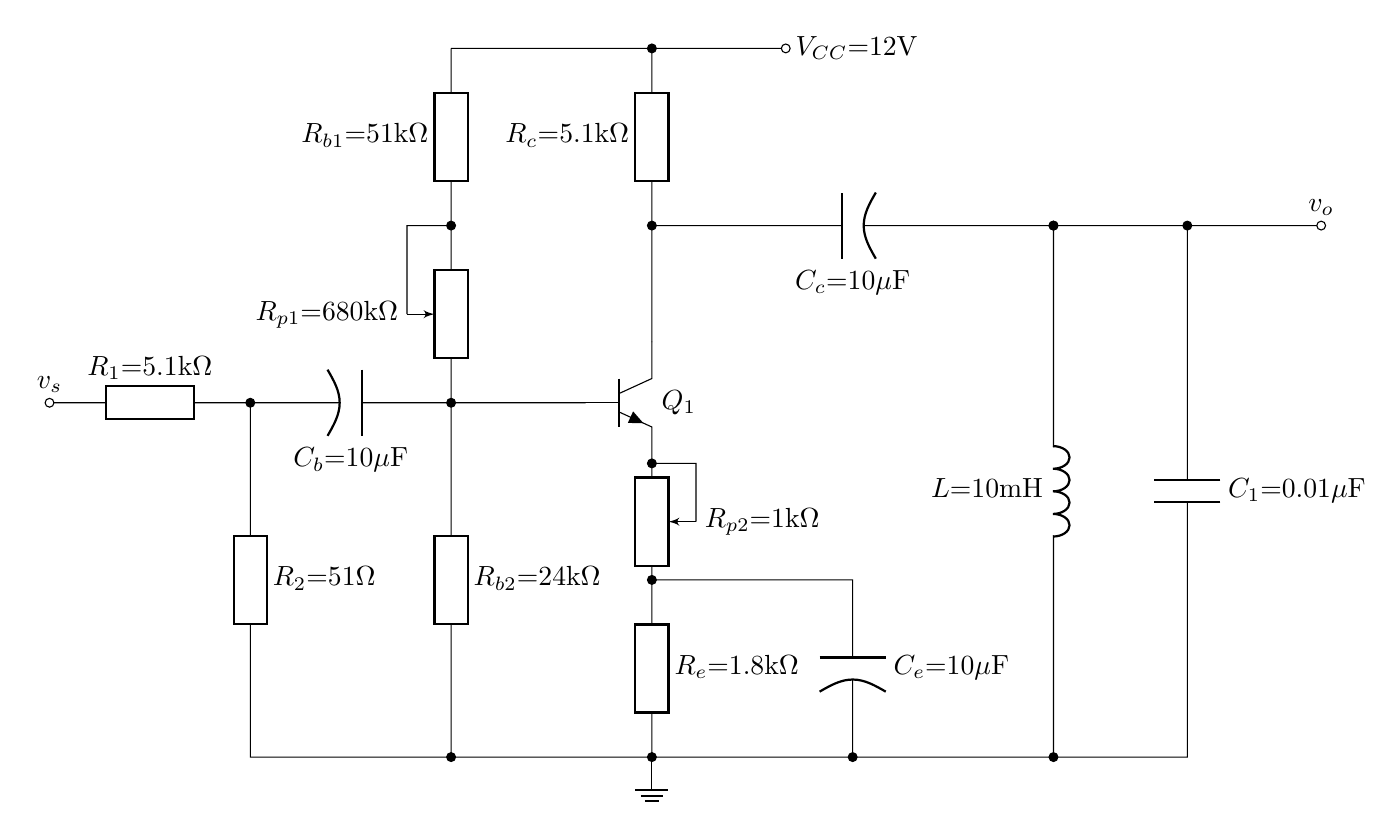
\begin{tikzpicture}[x = 1.7cm, y = 1.5cm]
    \draw
        (0,3) node[anchor = south]{$v_s$} to [R, l = $R_1{=}5.1\text{k}\Omega$, o-*] (1.5,3)
        (1.5,3) to [R, l = $R_2{=}51\Omega$] (1.5,0) -- ++(1.5,0) node[circ]{}
        (1.5,3) to [pC, l_= $C_b{=}10\mu\text{F}$] (3,3) node[circ]{} to [R, l = $R_{b2}{=}24\text{k}\Omega$] (3,0)
        (3,3) to [pR, l = $R_{p1}{=}680\text{k}\Omega$, n = PR1, -*] (3,4.5) to [R, l = $R_{b1}{=}51\text{k}\Omega$] (3,6)
        (3,4.5) -| (PR1.wiper)
        (4.5,3) node[npn](NPN){}
        (3,3) to [-] (NPN.B)
        (NPN.E) to [pR, l = $R_{p2}{=}1\text{k}\Omega$, n = PR2] (4.5, 1.5) to [R, l = $R_{e}{=}1.8\text{k}\Omega$] (4.5,0)
        (PR2.wiper) |- (NPN.E) node[circ]{}
        (NPN.C) to [-] (4.5,4.5) to [R, l = $R_c{=}5.1\text{k}\Omega$] (4.5,6) to [-] (3,6)
        (4.5,6) to [short, *-o] (5.5,6) node[right]{$V_{CC}{=}12\text{V}$}
        (7.5,4.5) to [pC, *-*, l = $C_c{=}10\mu\text{F}$] (4.5,4.5)
        (7.5,4.5) to [short, *-*] (8.5,4.5) to [C, l=$C_1{=}0.01\mu\text{F}$] (8.5,0) to [short, -*] ++(-1,0)
        (8.5,4.5) to [short, -o] (9.5,4.5)
        (7.5,4.5) to [american inductor, l_= $L{=}10\text{mH}$] (7.5,0)
        (6,0) to [pC, l_= $C_e{=}10\mu\text{F}$] (6,1.5) -- ++(-1.5,0) node[circ]{}
        (3,0) to [short, -*] (4.5,0) to [short, -*] (6,0) to [-] (7.5,0)
        (4.5,0) node[ground](GND){}
        {[anchor = south] (9.5,4.5) node{$v_o$}}
        {[anchor = west] (4.5,3) node{$Q_1$}}
    ;
    \end{tikzpicture}
\caption{LC选频放大电路}\label{fig3}   
\end{figure}

与前一节实验的电路相比,两者的差别是:前一节的电路的集电极仅接了电阻负载,为宽带放大器;本电路的集电极接的是并联调谐回路,为选频窄带放大器。
\iffalse
\begin{figure}[!h]
\centering
\subfloat[]{\label{fig4-1}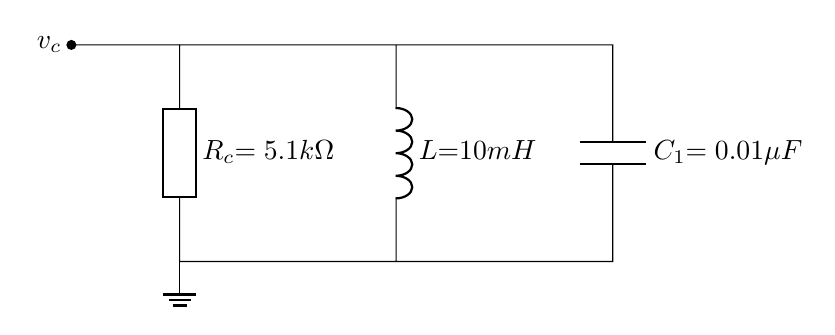
\begin{tikzpicture}[x = 2.75cm, y = 2.75cm]
    \draw
    (1,0) -- (2,0) to [C, l_ = $C_1{=0.01}\mu{F}$] (2,1) -- (1,1) to [american inductor, l = $L{=}10mH$] (1,0) -- (0,0) to [R, l_ = $R_c{=5.1k}\Omega$] (0,1) -- (1,1);
    \draw
    (0,1) to [short, -*] (-0.5,1);
    \draw
    (0,0) node[ground]{}
    (-0.5,1) node[anchor=east]{$v_c$};
\end{tikzpicture}}
\subfloat[]{\label{fig4-2}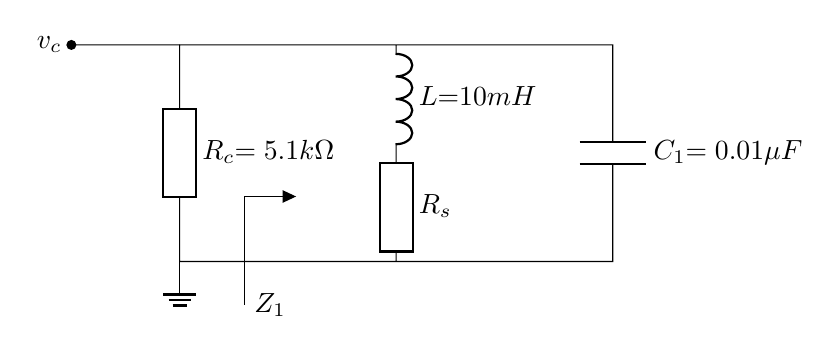
\begin{tikzpicture}[x = 2.75cm, y = 2.75cm]
    \draw
    (1,0) -- (2,0) to [C, l_ = $C_1{=0.01}\mu{F}$] (2,1) -- (1,1) to [american inductor, l = $L{=}10mH$] (1,0.5) to [R, l^ = $R_s$] (1,0) -- (0,0) to [R, l_ = $R_c{=5.1k}\Omega$] (0,1) -- (1,1);
    \draw
    (0,1) to [short, -*] (-0.5,1);
    \draw
    (0.3,-0.2) -- (0.3,0.3) -- (0.5,0.3) to node[currarrow,rotate=0]{} (0.5,0.3);
    \draw
    (0,0) node[ground]{}
    (-0.5,1) node[anchor=east]{$v_c$}
    (0.3,-0.2) node[anchor=west]{$Z_1$};
\end{tikzpicture}}
\subfloat[]{\label{fig4-3}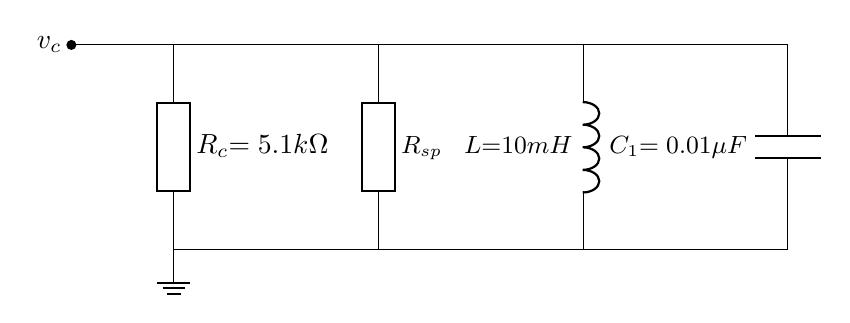
\begin{tikzpicture}[x = 2.6cm, y = 2.6cm]
    \draw
    (2,0) -- (3,0) to [C, l^ =\small $C_1{=0.01}\mu{F}$] (3,1) -- (2,1) to [american inductor, l_ =\small $L{=}10mH$] (2,0) -- (1,0) -- (0,0) to [R, l_ = $R_c{=5.1k}\Omega$] (0,1) -- (1,1) to [R, l =\small $R_{sp}$] (1,0);
    \draw
    (1,1) -- (2,1);
    \draw
    (0,1) to [short, -*] (-0.5,1);
    \draw
    (0,0) node[ground]{}
    (-0.5,1) node[anchor=east]{$v_c$};
\end{tikzpicture}}
\subfloat[]{\label{fig4-4}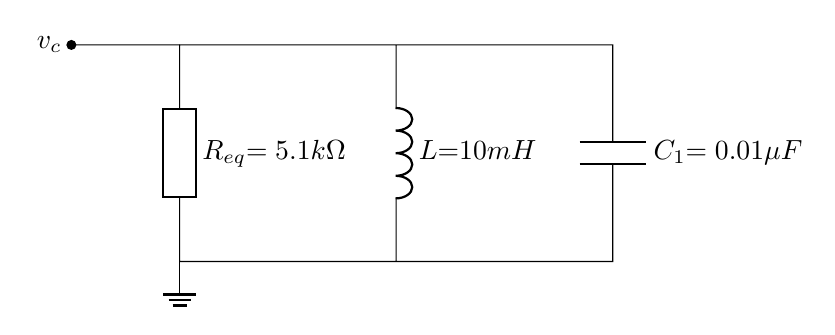
\begin{tikzpicture}[x = 2.75cm, y = 2.75cm]
    \draw
    (1,0) -- (2,0) to [C, l_ = $C_1{=0.01}\mu{F}$] (2,1) -- (1,1) to [american inductor, l = $L{=}10mH$] (1,0) -- (0,0) to [R, l_ = $R_{eq}{=5.1k}\Omega$] (0,1) -- (1,1);
    \draw
    (0,1) to [short, -*] (-0.5,1);
    \draw
    (0,0) node[ground]{}
    (-0.5,1) node[anchor=east]{$v_c$};
\end{tikzpicture}}
\caption{test}\label{fig4}
\end{figure}
\fi

\begin{figure}[!h]
    \subfloat{
    \begin{minipage}[!h]{0.4\textwidth}
    \begin{tikzpicture}[x = 2.6cm, y = 2.6cm]
    \draw
    (1,0) -- (2,0) to [C, l_ =\footnotesize $C_1{=0.01}\mu{F}$] (2,1) -- (1,1) to [american inductor, l =\footnotesize $L{=}10mH$] (1,0) -- (0,0) to [R, l_ =\footnotesize $R_c{=5.1k}\Omega$] (0,1) -- (1,1);
    \draw
    (0,1) to [short, -*] (-0.5,1);
    \draw
    (0,0) node[ground]{}
    (-0.5,1) node[anchor=east]{$v_c$};
    \end{tikzpicture}
    \caption*{(1)}\label{fig4-1}
    \end{minipage}
    }\qquad\qquad
    \subfloat{
    \begin{minipage}[!h]{0.4\textwidth}
    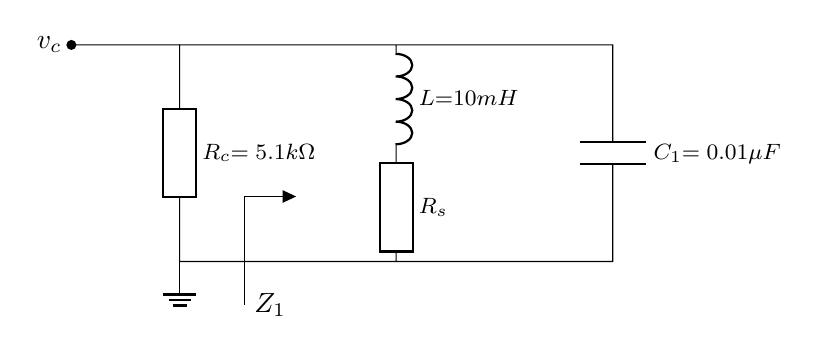
\begin{tikzpicture}[x = 2.75cm, y = 2.75cm]
    \draw
    (1,0) -- (2,0) to [C, l_ =\footnotesize $C_1{=0.01}\mu{F}$] (2,1) -- (1,1) to [american inductor, l =\footnotesize $L{=}10mH$] (1,0.5) to [R, l^ =\footnotesize $R_s$] (1,0) -- (0,0) to [R, l_ =\footnotesize $R_c{=5.1k}\Omega$] (0,1) -- (1,1);
    \draw
    (0,1) to [short, -*] (-0.5,1);
    \draw
    (0.3,-0.2) -- (0.3,0.3) -- (0.5,0.3) to node[currarrow,rotate=0]{} (0.5,0.3);
    \draw
    (0,0) node[ground]{}
    (-0.5,1) node[anchor=east]{$v_c$}
    (0.3,-0.2) node[anchor=west]{$Z_1$};
    \end{tikzpicture}
    \caption*{(2)}\label{fig4-2}
    \end{minipage}
    }
    \vfill
    \subfloat{
    \begin{minipage}[!h]{0.4\textwidth}
    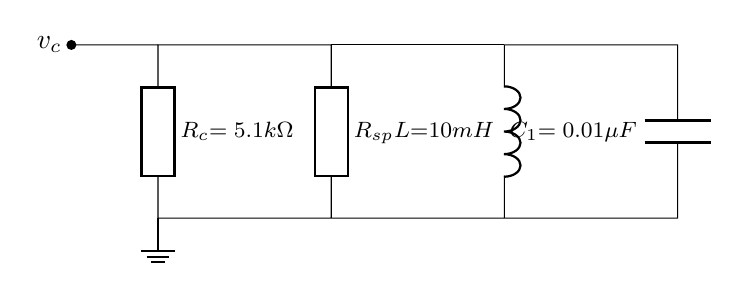
\begin{tikzpicture}[x = 2.2cm, y = 2.2cm]
    \draw
    (2,0) -- (3,0) to [C, l^ =\footnotesize $C_1{=0.01}\mu{F}$] (3,1) -- (2,1) to [american inductor, l_ =\footnotesize $L{=}10mH$] (2,0) -- (1,0) -- (0,0) to [R, l_ =\footnotesize $R_c{=5.1k}\Omega$] (0,1) -- (1,1) to [R, l =\footnotesize $R_{sp}$] (1,0);
    \draw
    (1,1) -- (2,1);
    \draw
    (0,1) to [short, -*] (-0.5,1);
    \draw
    (0,0) node[ground]{}
    (-0.5,1) node[anchor=east]{$v_c$};
    \end{tikzpicture}
    \caption*{(3)}\label{fig4-3}
    \end{minipage}
    }\qquad\qquad
    \subfloat{
    \begin{minipage}[!h]{0.4\textwidth}
    \begin{tikzpicture}[x = 2.6cm, y = 2.6cm]
    \draw
    (1,0) -- (2,0) to [C, l_ =\footnotesize $C_1{=0.01}\mu{F}$] (2,1) -- (1,1) to [american inductor, l =\footnotesize $L{=}10mH$] (1,0) -- (0,0) to [R, l_ =\footnotesize $R_{eq}{=5.1k}\Omega$] (0,1) -- (1,1);
    \draw
    (0,1) to [short, -*] (-0.5,1);
    \draw
    (0,0) node[ground]{}
    (-0.5,1) node[anchor=east]{$v_c$};
    \end{tikzpicture} 
    \caption*{(4)}\label{fig4-4}
    \end{minipage}
    }
    \caption{图(\ref{fig3})所示的选频放大器的输出回路}\label{fig4}
\end{figure}

对于交流信号,集电极接的LC$_1$并联调谐回路如图(\ref{fig4}-(1))所示。由于电感有损耗,实际电感可等效为一个无损耗电感$L_1$和一个等效电阻$R_s$的串联,如图(\ref{fig4}-(2))所示。$L_1$,$R_s$,$C_1$,的等效阻抗为
\begin{equation}
Z_1 = \cfrac{(R_s+j\omega L_1)\frac{1}{j\omega C_1})}{R_s+j\omega L_1+\frac{1}{j\omega C_1}} = \cfrac{\frac{L_1}{C_1}}{R_s+j\omega L_1+\frac{1}{j\omega C_1}} + \cfrac{\frac{R_s}{j\omega C_1}}{R_s+j\omega L_1+\frac{1}{j\omega C_1}}\label{eq3}
\end{equation}
记$\omega_0 = \frac{1}{\sqrt{L_1C_1}}$,$\frac{j\omega_0 L_1}{R_s}\left(\frac{\Omega}{\Omega_0} - \frac{\Omega_0}{\Omega}\right) = \xi$为广义失谐,$R_{sp} = \frac{L_1}{R_sC_1}$,$X_{C_1} = \frac{1}{\Omega C_1}$,
\begin{equation}
Z_1 = \cfrac{R_{sp}}{1+j\xi} - \cfrac{jX_{C_1}}{1+j\xi} = \cfrac{R_{sp} - \xi X_{C_1}}{1+\xi^2} + j\cfrac{-R_{sp}-X_{C_1}}{1+\xi^2}\label{eq4}
\end{equation}
回路谐振时,$Z_1$虚部为0,由$X_{C_1} = -R_{sp}\xi$可得谐振频率
\begin{equation}
\Omega_{o1} = \sqrt{\Omega^2_o - \frac{R_s^2}{L_1^2}} = \Omega_o\sqrt{1-\frac{R_s^2C_1}{L_1}} = \Omega_0\sqrt{1-\frac{1}{Q_1^2}}\label{eq5}
\end{equation}
其中$Q_1 = \frac{1}{R_s}\sqrt{\frac{L_1}{C_1}}$为$L_1C_1$谐振回路的品质因数。当$L_1C_1$回路的品质因数较大时,回路的谐振频率$\Omega_{o1} \approx \Omega_0$。当$\Omega = \Omega_{o1}$时,$Z_1$的虚部为0,用$X_{C_1} = -R_{sp}\xi$代入(1-8-4)式,可得$Z_1$实部
\begin{equation}
Z_1 = R_{sp} = \cfrac{L_1}{R_sC_1}\label{eq6}
\end{equation}

现在可将图(\ref{fig4}-(2))改画成图(\ref{fig4}-(3)).将$R_{sp}$与$R_c$并联,就得到了图(\ref{fig4}-(4))。

当输入信号频率为$L_1C_1$并联谐振频率$\Omega_{o1}$时,$L_1C_1$回路因谐振而等效为开路,放大器的集电极负载等效为纯阻,集电极阻抗最大,为图(\ref{fig4}-(4))中的$R_{eq}$,放大器放大倍数最大。若输入信号频率偏离$L_1C_1$并联谐振频率$\Omega_{o1}$,$L_1C_1$回路因失谐而不再等效为开路。集电极阻抗下降,放大器放大倍数下降,从而实现选频放大。

在本实验中,可测量$f_L$,$f_H$。记谐振时电路的输出电压幅值为$V_{o1}$,频率为$f_{o1}$;保持输人信号的幅值不变,降低其频率,当输出电压为0.707$V_{o1}$时的频率为$f_L$;再升高输人信号的频率,当输出电压再为0.707$V_{o1}$时的频率为$f_H$,电路的品质因数为
\begin{equation}
Q = \cfrac{f_{o1}}{f_H - f_L}\label{eq7}
\end{equation}
(\ref{eq7})式所示的品质因数是图(\ref{fig4}-(4))所示电路的品质因数。

由于Q可测得,$R_c$为已知,所以可以估算出电感的等效损耗电阻$R_{sp}$,$R_s$。设Q=4。
\begin{equation}
R_{eq} = Q\sqrt{\frac{L_1}{C_1}} = 4\times \sqrt{\frac{10\times 1-^{-3}}{0.01\times 10^{-6}}} = 4 (\text{k}\Omega)\label{eq8}
\end{equation}
由于$R_{eq} = R_c\parallel R_{sp}$,所以
\begin{equation}
R_{sp} = \cfrac{R_CR_{eq}}{R_C - R_{eq}} = \cfrac{5.1\times 4}{5.1 - 4} \approx 18.545 (\text{k}\Omega)\label{eq9}
\end{equation}
由(\ref{eq6})式可得电感的等效损耗电阻为
\begin{equation}
R_s = \cfrac{L_1}{R_{sp}C_1} = \cfrac{10\times 10^{-3}}{18545\times 0.01\times 10^{-6}} \approx 53.9 (\text{k}\Omega)\label{eq10}
\end{equation}
对于频率为$f_{o1}$的输入信号,电路的放大倍数为
\begin{eqnarray}
A_{V_{o1}} = -\cfrac{\beta R_{eq}}{r_{be}+(\beta +1)R_{p2}}\label{eq11}
\end{eqnarray}
\subsubsection{内容}
\begin{enumerate}
\item 按图(fig3)接线,将输人端短路,$R_{p2}$ = 100$\Omega$,调$R_{p1}$,使$V_C$ = 6V。
\item 用(\ref{eq8})式估箅$R_{eq}$,用(\ref{eq11})式估算$A_{V_{o1}}$.测量其幅频特性曲线,求其品质因数和谐振时的集电极等效负载电阻$R_{eq}$,电压放大倍数$A_{V{o1}}$。
\end{enumerate}

\section{实验数据}
\subsection{电容三端式LC振荡器}
\subsubsection{静态工作点}
$V_c$ = 6.016V,$R_P$ = 21.557k$\Omega$。
\subsubsection{$C_1$=10nF}
接上LC反馈回路后,测得输出信号的频率和峰峰值分别为:
$$f\text{ = 16.354kHz}$$
$$V_{PP} = 12.4\text{V}$$
波形图如图(\ref{datafig1})。
\begin{figure}[!h]
\centering
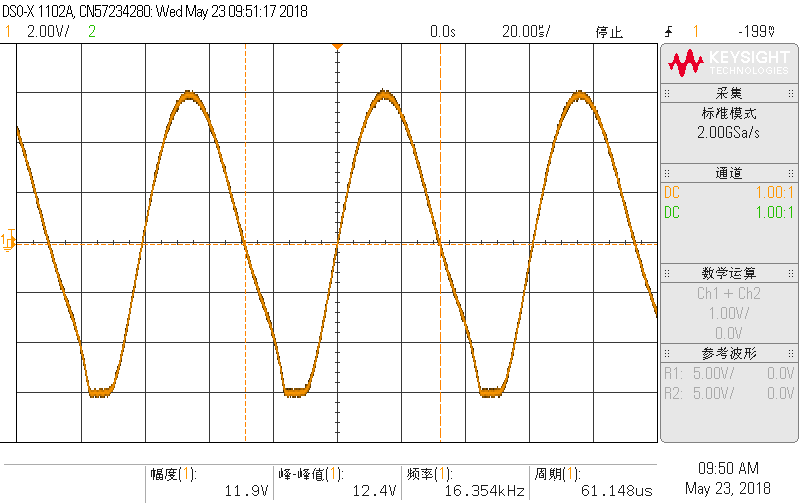
\includegraphics[width=10cm]{fig/scope_1.png}\\
\caption{未调节$R_{p2}$的波形图}\label{datafig1}
\end{figure}

调节$R_{p2}$后,波形改善。此时$R_{p2}$的阻值为:$R_{p2}\text{ = 133.877}\Omega$。波形图如图(\ref{datafig2})。
\begin{figure}[!h]
\centering
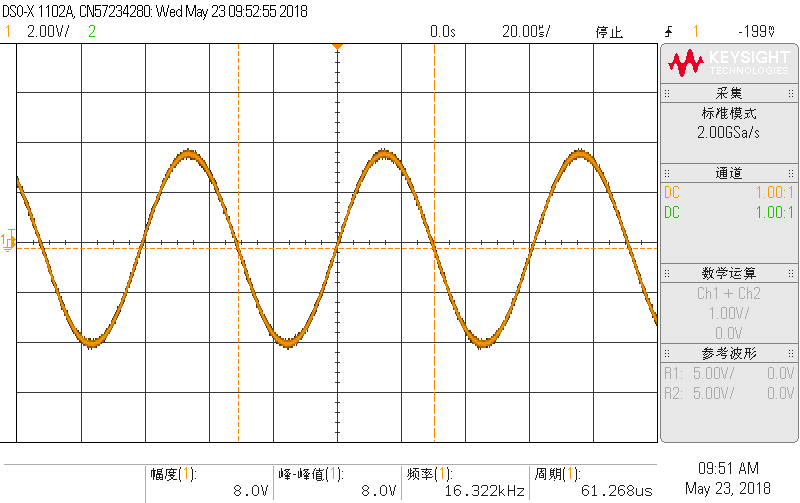
\includegraphics[width=10cm]{fig/scope_2.png}\\
\caption{调节$R_{p2}$后的波形图更加好看}\label{datafig2}
\end{figure}

\subsubsection{$C_1$=47nF}
将$C_1$改为47nF,重复上述步骤,数据如下:
$$f\text{ = 8.001kHz}$$
$$V_{PP}\text{ = 10.5V}$$
波形图如图(\ref{datafig3})。
\begin{figure}[!h]
\centering
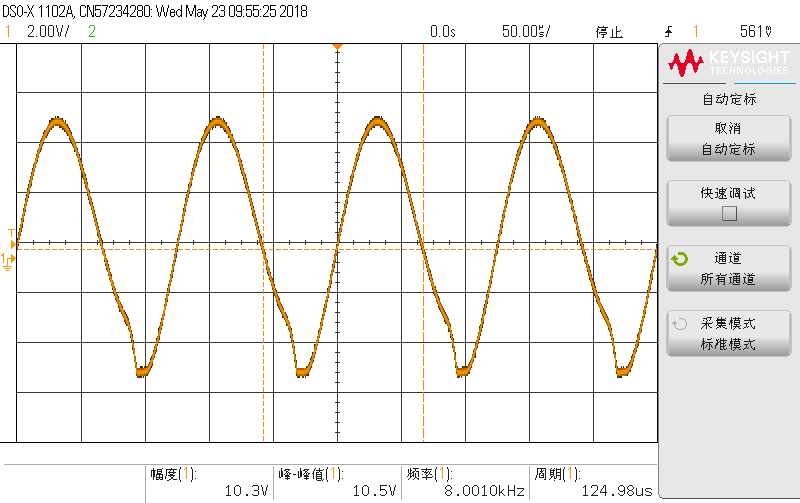
\includegraphics[width=10cm]{fig/scope_3.png}\\
\caption{未调节$R_{p2}$的波形图}\label{datafig3}
\end{figure}

调节$R_{p2}\text{ = 343.024}$,波形图改善,如图(\ref{datafig4})。
\begin{figure}[!h]
\centering
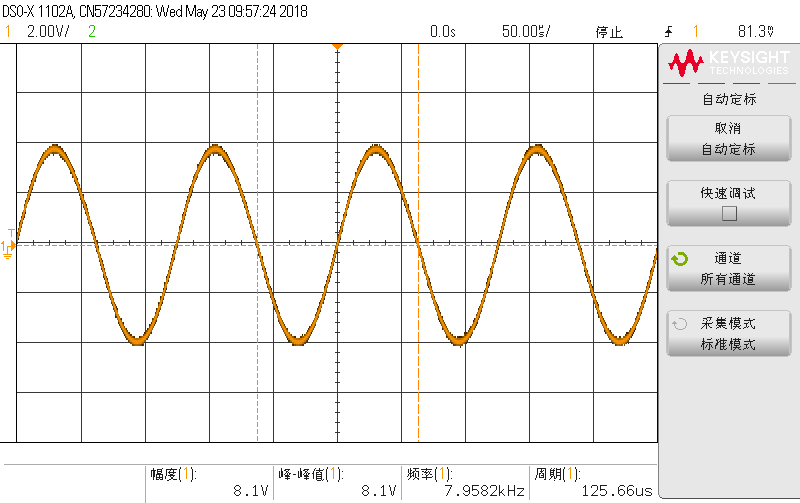
\includegraphics[width=10cm]{fig/scope_4.png}\\
\caption{调节$R_{p2}$后的波形图更加好看}\label{datafig4}
\end{figure}
\subsection{LC选频放大电路}
\subsection{静态工作点}
静态工作点数据如下:
$$R_{p2}\text{ = 100.666}\Omega$$
$$V_c\text{ = 6.0029V}$$
$$R_{p1}\text{ = 27.480k}\Omega$$
\subsection{幅频响应}
幅频响应数据如下:
输入电压为:$V_i$ = 9.655mV。

中频$f_o$ = 16kHz,此时的输出电压为$V_{orms}$ = 317.26mV。

低频截止频率为$f_L$ = 14.11kHz,高频截止频率为$f_H$ = 18.071kHz。

实验中我测量了LC选频放大电路的幅频响应,如图(\ref{AFCfig}):
\begin{figure}[!h]
\centering
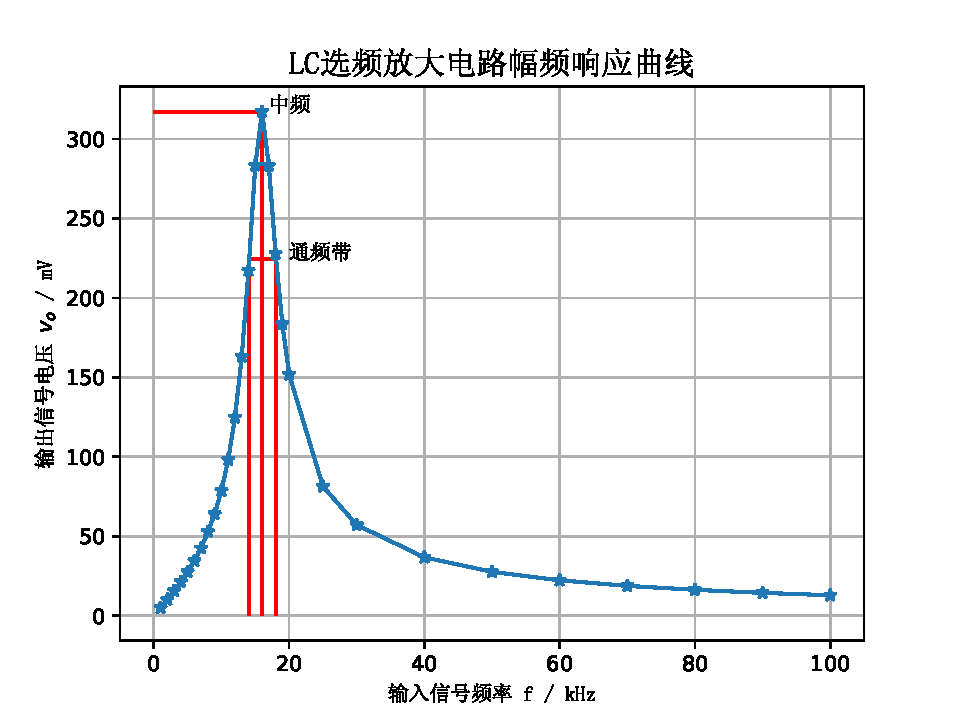
\includegraphics[width=12cm]{fig/AFC.pdf}\\
\caption{LC选频放大电路幅频响应}\label{AFCfig}
\end{figure}

相应的计算值为:
\begin{enumerate}
\item 品质因子:\\
\begin{equation}
Q = \cfrac{f_o}{f_H - f_L} = \cfrac{16}{18.071 - 14.112} \approx 4.0414\label{Q}
\end{equation}
\item 放大倍数\\
\begin{equation}
A = \cfrac{V_o}{V_i} = \cfrac{317.26}{9.655} \approx 32.86\label{A_V}
\end{equation}
\item 误差\\
中频的理论值为:
\begin{equation}
f_{ot} = \cfrac{1}{2\pi\sqrt{LC}} = \cfrac{1}{2\pi\sqrt{10\text{mH}\times 0.01\mu \text{F}}} \approx 15.915\text{ kHz}\label{fo_theory}
\end{equation}
所以误差为:
\begin{equation}
\text{Error\%} = \cfrac{f_o - f_{ot}}{f_{ot}} = \cfrac{16-15.915}{15.915}\times 100\% \approx 0.534\%\label{Error}
\end{equation}
\end{enumerate}

\section{实验讨论}
\subsection{静态工作点}
在实验过程中,发现调好的静态工作点会逐渐向一个方向漂移,使得实验前后的静态工作点往往不再一样,这可能会对放大器的工作产生一定影响。


\section{思考题}
\subsection{绘制图(\ref{fig1})所示电路的交流微变等效电路。}
\begin{figure}[!h]
\centering
\begin{circuitikz}[x = 2.25cm, y = 2.25cm]
    \draw
    (2,0) -- (3,0) to [C] (3,1) to [short,-*] (2,1) -- (2,0.8) -- (2.1,0.5) -- (2,0.2) -- (1.9,0.5) -- (2,0.8)
    (2,0.2) to [short,-*] (2,0) -- (1,0)
    (1,1) to [short, o-o] (0,1)
    (1,0) -- (0,0)
    (0,0) node[ground]{};
    \draw
    (3,1) to [short,*-o] (3.5,1)
    (3,1) to [short,-*] (3,1.1) -- (3.2,1.1) to [C] (3.2,1.9) -- (2.8,1.9) to [american inductor] (2.8,1.1) -- (3,1.1)
    (3,1.9) to [short,*-] (3,2) -- (0.5,2) to [short,-*] (0.5,1);
    \draw
    (0,1) node[anchor=east]{$v_i$}
    (3.5,1) node[anchor=west]{$v_o$};
\end{circuitikz}
\caption{图(\ref{fig1})交流微变等效电路}\label{question1}
\end{figure}
\subsection{图(\ref{fig1})所示电路起振时要求|$\dot{A}_V\dot{F}$|$>$1,稳态时要求
|$\dot{A}_V\dot{F}$|=1。试述该电路的电压放大倍数能自动调节,以满足上述要求。}
由前文可知:电路刚起振时,电路输出$v_o$较小。由于|$\dot{A}_V\dot{F}$|$>$1,信号在从输出端、经反馈到反相输人端、再到输出端的过程中被放大,集电极电压和电流不断被放大,电路输出$v_o$不断增大。在此过程中,集电极电流逐步被限幅,由于发射极PN结的非线性特性,使基极、发射极电流正半周幅值大,负半周幅值小,由此产生直流电流分量。直流电流分量对发射极旁路电容$C_e$充电, 使发射极直流电位上升,从面使$V_{BE}$下降,三极管Q的电流放大倍数下降,放大器A的放大倍数下降.这时电路达到|$\dot{A}_V\dot{F}$|=1,若出现
|$\dot{A}_V\dot{F}$|$<$1,即集电极电流减小,输出电压减小,则由于发射极PN结的非线性特性产生的直流电流减小,发射极电容上的直流电位减小,从而使$V_{BE}$上升,三极管$Q_1$的电流放大倍数$\beta$上升,放大器A的放大倍数增大,电路重新回到|$\dot{A}_V\dot{F}$|=1。称这种性能为自动稳幅性能。
\subsection{您在实验中使用什么方法减小图(\ref{fig1})所示电路输出波形的谐波失真?试分析其原因。}
\begin{enumerate}
\item 减小$C_1$\\
观察图(\ref{datafig1})和图(\ref{datafig3})可以看出,$C_1$较小的情况下,输出波形的谐波失真较小。
\item 改变$R_{p2}$\\
观察图(\ref{datafig1})和图(\ref{datafig2})可以看出,调节$R_{p2}$后输出波形明显改善。
\end{enumerate}
\subsection{试述晶体管低频等效电路与高频等效电路的主要差别。若减小L,$C_1$的数值,电路的谐振频率将受到什么因素的制约?}
低频放大器工作频率低,通频带宽;高频放大器工作频率高,通频带窄,有中心频率和选频作用。由于电容和电感的存在,低频电路容抗高、感抗低;高频电路容抗低、感抗高。

若减小L,$C_1$的值,则中频会增大。中频还会受到三极管内禀参数和静态工作点的影响。

\nocite{jiaocai}
%--------bib------------------
\bibliography{ref}
\end{document}